\documentclass[12pt,oneside,noprintercorrection]{iut}
\usepackage[utf8]{inputenc}
%----------------------------------------------------------------------
%                     Chargement de quelques packages
%----------------------------------------------------------------------

% Si l'on produit le PDF avec pdflatex, ceci remplace la plupart
% des polices EC par des polices CM, plus adaptees a la generation de PDF,
% car ayant des equivalents PS :

\usepackage[cyr]{aeguill}

% pour les includegraphics
\usepackage{graphicx}

% mini "table of content"
\usepackage[french]{minitoc}
\usepackage[french]{babel}


% couleur des liens et hyperref -> mettre à {0.0,0.0,0.0} pour avoir du noir
%                               -> mettre à {0.2,0.2,0.2} pour avoir du gris foncé
\usepackage{color}
\definecolor{linkcolor}{rgb}{0.1,0.1,0.7}
\usepackage[hypertexnames=false]{hyperref}
\hypersetup{
    colorlinks,%
    citecolor=linkcolor,%
    filecolor=linkcolor,%
    linkcolor=linkcolor,%
    urlcolor=linkcolor,%
}

% Pour les codes
\usepackage{listings}
\lstset{language=C++,basicstyle=\small}


\usepackage{silence}

\WarningFilter{minitoc(hints)}{W0023}
\WarningFilter{minitoc(hints)}{W0024}
\WarningFilter{minitoc(hints)}{W0028}
\WarningFilter{minitoc(hints)}{W0030}
\WarningFilter{hyperref}{bookmark level}

\WarningFilter{blindtext}{} % this takes care of the `blindtext` messages

%-------------------------------------------------------------------
%  Surcharge de commandes pour les variables et page d'en-tête
%-------------------------------------------------------------------

\makeatletter

%
% les deux commandes suivantes sont entre \makeatletter
% et \makeatother parce qu'elles utilisent des `@'.
%

\renewcommand{\@DFD}{Universit\'e Polytechnique des Hauts de France\\}


\renewcommand{\@Lillehe@d}{{\UseEntryFont{ThesisFirstPageHead}\noindent
    \centerline{\if@logo@uhp@
                    {\setbox0=\hbox{$\raise2.3cm\hbox{\UHPLogo}$}%
                     \ht0=\baselineskip\box0}\hfill
                \else
                    Universit\'e Lille%
                \fi}%
    \@TL@cmn@head\\
    \par
    }%
    }


\newcommand\TheseLilleI{\renewcommand{\@ThesisFirstPageHead}{\@Lillehe@d}%
                         \ThesisDiploma{{\UseEntryFont{ThesisDiploma}%
                              \\[3mm]
            {\UseEntryFont{ThesisSpecialty}( )}}}}

\makeatother

%-------------------------------------------------------------------
%           Corrections pour les imprimantes recto-verso
%                          (A AJUSTER)
%-------------------------------------------------------------------

%\ShiftOddPagesRight{-1mm}
%\ShiftOddPagesDown{2.5mm}
%\ShiftEvenPagesRight{0mm}
%\ShiftEvenPagesDown{0mm}

%-------------------------------------------------------------------
%                Mise en page
%-------------------------------------------------------------------

%-------------------------------------------------------------------
%                             interligne
%-------------------------------------------------------------------
\renewcommand{\baselinestretch}{1.3}

%-------------------------------------------------------------------
%                             Marges
%-------------------------------------------------------------------

% pour positionner les vraies marges:
%\SetRealMargins{1mm}{1mm}

%-------------------------------------------------------------------
%                             En-tetes
%-------------------------------------------------------------------
%On n'utilise pas les logos
%\DontShowLogos

% Les en-tetes: quelques exemples
%\UppercaseHeadings
%\UnderlineHeadings
%\newcommand\bfheadings[1]{{\bf #1}}
%\FormatHeadingsWith{\bfheadings}
%\FormatHeadingsWith{\uppercase}
%\FormatHeadingsWith{\underline}
\newcommand\upun[1]{\uppercase{\underline{\underline{#1}}}}
\FormatHeadingsWith\upun

\newcommand\itheadings[1]{\textit{#1}}
\FormatHeadingsWith{\itheadings}

% pour avoir un trait sous l'en-tete:
\setlength{\HeadRuleWidth}{0.4pt}


%-------------------------------------------------------------------
%                         Les references
%-------------------------------------------------------------------

\NoChapterNumberInRef \NoChapterPrefix

%-------------------------------------------------------------------
%                           Brouillons
%-------------------------------------------------------------------

% ceci ajoute une marque `brouillon' et la date
%\ThesisDraft




\renewcommand{\labelitemi}{$\bullet$}
\renewcommand{\labelitemii}{$\circ$}
%-------------------------------------------------------------------
%                          Encadrements
%-------------------------------------------------------------------

% encadre les chapitres dans la table des matieres:
% (ces commandes doivent figurer apres \begin{document}

%\FrameChaptersInToc
%\FramePartsInToc


%-------------------------------------------------------------------
%            Reinitialisation de la numerotation des chapitres
%-------------------------------------------------------------------

% Si la commande suivante est presente,
% elle doit figurer APRES \begin{document}
% et avant la premiere commande \part
\ResetChaptersAtParts

%-------------------------------------------------------------------
%               mini-tables des matieres par chapitre
%-------------------------------------------------------------------

% preparer les mini-tables des matieres par chapitre.
% (commande de minitoc.sty)
%\dominitoc

\NewJuryCategory{EncadrantEts}{\it Encadrant entreprise :}{\it Encadrant entreprise:} 
\NewJuryCategory{EncadrantUniv}{\it Encadrant universitaire :}{\it Encadrant universitaire:} 

\TheseLilleI


% Commandes macros de raccourcis
\newcommand{\glaz}{Glaz tech+fi}
\newcommand{\gz}{Glaz}
\newcommand{\slf}{Salesforce}
\newcommand{\fa}{Form Assembly}




%-------------------------------------------------------------------
%                         Page de titre:
%-------------------------------------------------------------------


\ThesisTitle{Aider les analystes financiers à numériser leur travail avec Salesforce}
\ThesisKind{Rapport de stage}
\ThesisPresentedThe{soutenu le 27/06/2023}
\ThesisAuthor{Sacha DON}

\NomDuLaboOuEntreprise{\glaz{}}
\LogoLaboOuEntreprise{img/logoglaz.png} % Image du logo du labo ou ets dans le rep img

\EncadrantEts = {Antoine Laudet}
\EncadrantUniv = {Mustapha Ratli}

\begin{document}

% Creation de la page de titre:
\MakeThesisTitlePage



%-------------------------------------------------------------------


%-------------------------------------------------------------------
%                          remerciements
%-------------------------------------------------------------------

%\DontFrameThisInToc
\begin{ThesisAcknowledgments}
Je voudrais avant tout remercier toute l'équipe de \glaz{}. Notamment Monsieur Samuel MINNE, le CTO, Quentin PROGNON, alternant en Master E-Services et chef du projet sur lequel j'ai travaillé, il m'a aidé à m'améliorer en tant que développeur mais il m'a également été d'une aide précieuse pour la rédaction de ce rapport. Je tiens également à remercier Zo Tahina RATEFIARIVONY, alternant en Master Génie Logiciel, Louise DELBECQUE, alternante en Master E-Services, Abdelkader AMARA, alternant en Master E-Services également, Anis SAHED, alternant en MIAGE, Kenneth MAGNAGNA, alternant en études de finance de marché trading, Néo LEFRANC, stagiaire en Licence Informatique et Antoine LAUDET, le dirigeant de l'entreprise, qui m'ont fait confiance, m'ont gracieusement accueilli mais qui m'ont surtout encadré et aidé tout au long de cette année d'alternance.
J'aimerais également remercier Monsieur Mustapha RATLI qui m'a suivi durant cette année d'alternance.
\end{ThesisAcknowledgments}





%-------------------------------------------------------------------
%                  ecriture de `Chapitre' et `Partie'
%                      dans la table des matieres
%-------------------------------------------------------------------

\WritePartLabelInToc \WriteChapterLabelInToc


%-------------------------------------------------------------------
%                        table des matières
%-------------------------------------------------------------------

\tableofcontents

%-------------------------------------------------------------------
%              Exemple d'utilisation de \SpecialSection
%-------------------------------------------------------------------

% La commande \mainmatter (nouvelle commande LaTeX2e) permet de passer
% a la numérotation arabe (ce que fait \pagenumbering{arabic})
% et de faire commencer la nouvelle page 1 sur une page impaire.
% On evitera donc d'utiliser directement \pagenumbering{arabic}.
\mainmatter

% ----------------------------------------------------------------
\SpecialSection{Introduction}
Dans le cadre de ma formation en Licence professionnelle Développement Web et Mobile, j'ai eu l'opportunité d'effectuer une alternance au sein de l'entreprise \glaz{}. Cette expérience m'a permis de mettre en pratique les connaissances acquises lors de ma formation, mais aussi de développer de nouvelles compétences en travaillant sur des projets concrets et stimulants.

L'entreprise Glaz Tech +Fi est spécialisée dans le développement de solutions technologiques innovantes. Parmi ses réalisations, le Shaker Data se distingue comme un outil essentiel de l'entreprise. C'est un véritable allié pour les professionnels du secteur financier, tels que les analystes financiers, les gestionnaires de patrimoine ou encore les courtiers immobiliers. Le Shaker Data est conçu pour recueillir et analyser les informations des clients, permettant ainsi d'évaluer la faisabilité de crédits bancaires. L'objectif est de proposer des produits bancaires sur mesure, parfaitement adaptés aux besoins spécifiques de chaque client.

Durant mon alternance, j'ai eu le privilège de contribuer au développement et à la maintenance du Shaker Data. Cette expérience m'a permis non seulement de comprendre le fonctionnement interne de cet outil, mais aussi de participer activement à son amélioration et à son évolution.

Ce rapport présente en détail les activités que j'ai menées au cours de mon alternance, les compétences que j'ai acquises et les leçons que j'ai tirées de cette expérience enrichissante.

Dans la première partie de ce rapport, je présenterai Glaz Tech +Fi puis j'expliquerai en détail le rôle du Shaker Data au sein de l'entreprise. Ensuite, je décrirai la méthode et les moyens que j'ai utilisés pour développer et maintenir l'outil. La troisième partie sera consacrée à la présentation des résultats de mon travail et des apports de celui-ci. Enfin, je conclurai en soulignant les contributions significatives de mon travail à l'entreprise, en mettant en évidence les compétences et les connaissances que j'ai acquises au cours de cette expérience.

% Pour ne paœur du s avoir le mot `Chapitre' au debut de chaque chapitre.
\NoChapterHead

\chapter{Comprendre \glaz{} et le Rôle du Shaker Data}
\section{\glaz{}}

\glaz{}, forte de plus de 20 ans d'expertise en solutions financières, a su s'adapter aux évolutions technologiques et informatiques pour se réinventer en tant que Fintech. Collaborant avec des acteurs financiers tels que des gestionnaires de patrimoine, des analystes financiers et des courtiers immobiliers, l'entreprise a réussi à numériser ses processus métiers grâce à l'intégration de Salesforce. Cette transformation a marqué un tournant significatif pour Glaz Tech +Fi, qui a su allier avec brio l'analyse financière et l'informatique.

\gz{} se consacre à fournir à ses clients des solutions financières adaptées à leurs besoins spécifiques de financement. Pour atteindre cet objectif, l'entreprise a établi plusieurs mandats avec diverses banques. Ces mandats permettent non seulement à Glaz Tech +Fi de proposer des solutions financières personnalisées à ses clients, mais aussi de comprendre en profondeur les spécificités de chaque produit financier.

En tant que mandataire de banque, le rôle de \glaz{} est d'accompagner ses clients tout au long de leur parcours de financement. Cela comprend la préparation du dossier de financement jusqu'à la signature finale du contrat.

Actuellement, \gz{}, en tant que mandataire de banque, propose des solutions de financement pour trois types de projets principaux : les projets de financement immobilier, le rachat de crédit, et l'acquisition de parts de Sociétés Civiles de Placement Immobilier (SCPI).

L'entreprise se compose de deux équipes complémentaires : une équipe financière et commerciale basée à Ploemeur, en Bretagne, et une équipe informatique située à Lille. Cette configuration permet une communication constante et efficace entre les deux équipes, essentielle pour définir conjointement les besoins, suivre les évolutions et corriger les éventuels bugs.

Glaz Tech +Fi se distingue par son processus d'analyse de dossiers de financement provenant d'apporteurs d'affaires, notamment des conseillers en gestion de patrimoine, des courtiers immobiliers, ou bien des analystes financiers. Une fois le dossier reçu, l'entreprise réalise une analyse approfondie de sa faisabilité. La qualité de cette analyse est largement reconnue, tant par les apporteurs d'affaires que par les banques partenaires, attestant de l'expertise et de la fiabilité de Glaz Tech +Fi.


\subsection{La transformation digitale de \gz{}}

Il y a cinq ans, Glaz Tech +Fi a choisi de diversifier ses activités en créant une branche dédiée au développement informatique, se positionnant ainsi en tant que \textit{fintech}. Cette nouvelle branche, basée à Lille, est responsable du développement de tous les outils informatiques utilisés par Glaz Tech +Fi. Ces outils sont conçus pour être utilisés non seulement par toutes les équipes de Glaz Tech +Fi, mais aussi par ses collaborateurs.

En plus de cela, Glaz Tech +Fi a décidé d'étendre son champ d'action en développant des outils informatiques destinés à d'autres entreprises ainsi qu'aux particuliers.

\clearpage

\section{Le Shaker Data}
L'outil principal de Glaz Tech +Fi est le Shaker Data. C'est un outil numérique conçu pour gérer de manière exhaustive le processus de création d'un dossier de financement. Auparavant, les analystes financiers de Glaz Tech +Fi consacraient la majeure partie de leur temps à l'évaluation de la faisabilité d'un dossier de financement. Ce processus, qui impliquait l'analyse des spécificités de chaque produit financier pour chaque dossier, était long et laborieux pour l'équipe.

Le Shaker Data a transformé ce processus en numérisant l'ensemble du parcours, de la création du dossier de financement à la signature du contrat de financement. Une fois qu'un dossier de financement est saisi dans le Shaker Data, l'outil analyse automatiquement le dossier et propose une liste de solutions de financement adaptées aux besoins du client et de sa situation financière.

Cet outil apporte une valeur ajoutée significative à l'équipe financière de Glaz Tech +Fi. Il leur permet de se concentrer sur l'analyse des dossiers de financement tout en économisant le temps autrefois consacré à la gestion des dossiers papier. Avant l'introduction du ShakerData, l'évaluation de la faisabilité d'un dossier de financement pouvait prendre jusqu'à deux semaines, le temps nécessaire pour les analystes pour traiter le dossier et obtenir les réponses des banques.

\begin{figure}[!ht]
  \centering
  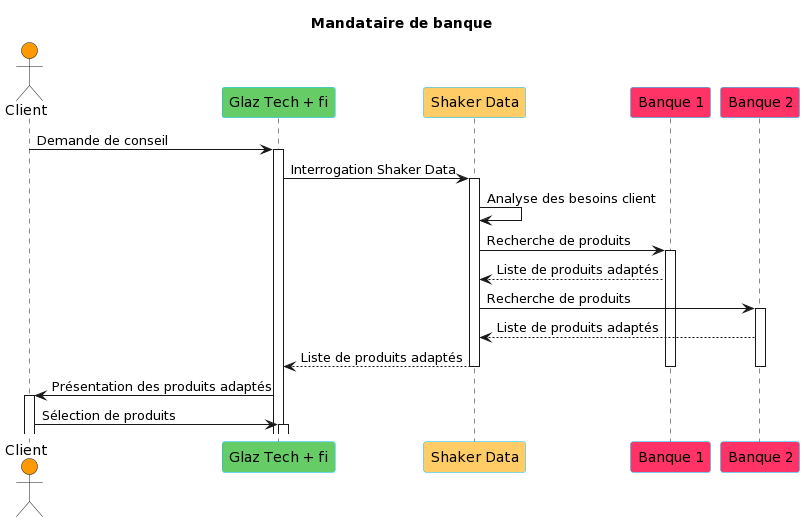
\includegraphics[width=12cm]{img/FonctionnementGlaz.png}
  \caption{Fonctionnement de \gz{}}
\end{figure}

\clearpage

Cependant, le monde financier étant en constante évolution, les produits financiers doivent subir des mises à jour régulières, et les banques doivent s'adapter non seulement aux fluctuations du marché, mais aussi aux contraintes légales qui leur sont imposées. Par conséquent, il est essentiel pour \glaz{} de maintenir une évolution constante de ses outils informatiques. Cela garantit qu'ils ne deviennent pas obsolètes en proposant des solutions de financement qui ne correspondent plus à la réalité actuelle du marché.
En tant que fintech émergente et en expansion, Glaz Tech +Fi est confrontée à plusieurs défis. Le premier défi consiste à faire évoluer ses outils informatiques afin qu'ils répondent au mieux aux besoins de ses clients. Le deuxième défi est de garantir que ses outils soient suffisamment efficaces et attrayants pour attirer de nouveaux clients. Le troisième défi est de s'assurer que ses outils peuvent répondre à une variété suffisante de besoins de financement, permettant ainsi à Glaz Tech +Fi de continuer à croître malgré la crise actuelle.

\section{Pourquoi cette alternance ?}
Ayant fait un stage au sein de cette entreprise l'an dernier dans le cadre de l'obtention d'un DUT Informatique, j'ai voulu poursuivre dans celle-ci en alternance afin de continuer à m'améliorer en tant que développeur, mais également pour acquérir du savoir-faire des technologies de \slf{}.

\chapter{\slf{} et ses technologies}

\slf{} est la plateforme de développement que \glaz{} a choisie pour développer ses outils. Actuellement, \slf{} est le leader du marché en ce qui concerne la facilitation des relations entre les entreprises et leurs clients. C'est aussi une plateforme de développement qui a été parmi les premières à promouvoir les \textit{SaaS} (Software as a Service) et le no-code.

\section{Le no-code sur \slf{}}
Le no-code est une approche de développement d'applications qui permet aux utilisateurs de créer des applications fonctionnelles sans avoir à écrire de code. Au lieu de cela, les utilisateurs peuvent utiliser des outils visuels pour concevoir l'interface utilisateur de l'application, définir la logique de l'application et même configurer des intégrations avec d'autres systèmes.

Dans le contexte de Salesforce, le no-code est une partie intégrante de la plateforme. Salesforce offre une variété d'outils no-code qui permettent aux utilisateurs de personnaliser leur instance Salesforce et de créer des applications personnalisées.

L'un des principaux avantages de l'approche no-code est qu'elle permet à des utilisateurs non techniques, comme l'équipe financière, de modifier le comportement des outils développés sans nécessiter l'intervention de l'équipe de développement. Cela peut aider à augmenter la productivité de l'équipe financière, car ils peuvent faire des ajustements et des modifications sans avoir à attendre que l'équipe de développement soit disponible. De plus, cela peut aider à réduire la charge de travail de l'équipe de développement, car ils n'ont pas à passer du temps à faire des modifications mineures qui pourraient être effectuées par l'utilisateur final.

En somme, l'approche no-code de Salesforce offre une flexibilité et une autonomie accrues aux utilisateurs, tout en permettant aux développeurs de se concentrer sur des tâches plus complexes et plus stratégiques.

\section{Les langages de \slf{}}

\subsection{Le langage Apex}
Apex est un langage de programmation fortement typé, orienté objet, qui permet aux développeurs d'ajouter une logique métier à des événements système, tels que des clics sur des boutons, des mises à jour d'enregistrements associés, et des pages Visualforce. Il utilise une syntaxe de type Java et agit de la même manière que des procédures stockées de base de données. Voici quelques caractéristiques clés d'Apex :

- Hébergé : Apex est enregistré, compilé et exécuté sur le serveur Lightning Platform de Salesforce.

- Orienté objet : Apex prend en charge les classes, les interfaces et l'héritage.

- Fortement typé : Apex valide des références à des objets lors de la compilation.

- Respectueux de la mutualisation : Le langage Apex, étant exécuté dans une plateforme mutualisée, empêche l'emballement du code en imposant des limitations qui évitent de monopoliser les ressources partagées.

- Intégré à la base de données : Il est extrêmement facile d'accéder à et de manipuler des enregistrements. Apex offre un accès direct aux enregistrements et à leurs champs, et fournit des instructions et des langages de requête pour manipuler ces enregistrements via le langage SOQL.

- Orienté vers les données : Apex offre un accès transactionnel à la base de données, qui permet de restaurer les opérations.

- Facile à utiliser : Apex est basé sur les idiomes Java habituels.

- Facile à tester : Apex fournit une prise en charge intégrée de création de tests unitaires, d'exécution et de couverture de code. Salesforce vérifie que tous les codes Apex personnalisés fonctionnent normalement, en exécutant tous les tests unitaires avant une mise à niveau de la plateforme. Afin de déployer, il faut obligatoirement avoir une couverture de code d'au moins 75\%.

En tant que développeur, vous pouvez écrire et déboguer du code Apex sur votre ordinateur client à l’aide des extensions Salesforce pour Visual Studio Code. Vous pouvez également écrire du code Apex et accéder aux informations de débogage directement dans le navigateur en utilisant l’interface utilisateur de Salesforce.

En résumé, Apex est un langage de programmation puissant qui permet aux développeurs de personnaliser les applications Salesforce au-delà de ce qui est possible avec les outils de configuration standard. Il offre une grande flexibilité et un contrôle précis sur la logique métier de votre application Salesforce.

\subsection{Le SOQL}

Salesforce Object Query Language (SOQL) est un langage de requête qui permet de rechercher vos données organisationnelles spécifiques à Salesforce. Il est similaire à SQL, le langage de requête standard utilisé pour interroger les bases de données, mais il est spécifiquement conçu pour Salesforce et contient des fonctionnalités supplémentaires adaptées à ses services.

Voici quelques caractéristiques clés de SOQL :

- Objets et champs : Dans Salesforce, nous avons des objets, qui sont équivalents aux tables de base de données en SQL. Nous avons également des champs, qui sont équivalents aux colonnes d'une base de données. Ensuite, nous avons des enregistrements, qui sont représentatifs des lignes dans la base de données.

- Syntaxe de requête : La syntaxe de base pour une requête SOQL est SELECT {fields} FROM {object} WHERE {condition}. C'est très similaire à la syntaxe SQL standard.

- Intégration avec Salesforce : SOQL est étroitement intégré avec la plateforme Salesforce. Vous pouvez exécuter des requêtes SOQL directement dans l'interface utilisateur de Salesforce, ou vous pouvez les exécuter à partir de code Apex.

- Limitations : Contrairement à SQL, SOQL ne supporte pas certaines fonctionnalités telles que les jointures arbitraires entre objets ou les sous-requêtes dans la clause FROM. Cependant, il supporte d'autres fonctionnalités utiles telles que les requêtes parent-enfant.

En tant que développeur, vous pouvez utiliser SOQL pour interroger vos données Salesforce, extraire des informations précises, créer des rapports et alimenter vos applications personnalisées avec des données précises.
\clearpage

\subsection{Le framework Visualforce}
Visualforce est un framework qui permet aux développeurs de créer des interfaces utilisateur personnalisées qui s'intègrent avec la plateforme Salesforce. Il permet aux développeurs de créer des pages, des composants et des applications sophistiquées avec des balises personnalisées et des contrôleurs Apex.

Voici quelques caractéristiques clés de Visualforce :

- Balises personnalisées : Visualforce utilise un ensemble de balises personnalisées fournies par Salesforce pour créer des interfaces utilisateur. Ces balises ressemblent à du HTML et peuvent être utilisées pour afficher ou travailler avec des données Salesforce.

- Contrôleurs Apex : Les contrôleurs Apex sont utilisés pour définir la logique personnalisée derrière les pages Visualforce. Ils peuvent être utilisés pour manipuler des données, naviguer entre les pages, et plus encore.

- Intégration avec Salesforce : Visualforce est étroitement intégré avec la plateforme Salesforce. Les pages Visualforce peuvent interagir avec des données Salesforce, utiliser des contrôleurs Apex pour la logique personnalisée, et être intégrées dans l'interface utilisateur standard de Salesforce.

- Personnalisation : Avec Visualforce, vous pouvez créer des interfaces utilisateur hautement personnalisées qui vont au-delà de ce qui est possible avec les outils de configuration standard de Salesforce. Vous pouvez contrôler l'apparence et le comportement de vos pages avec une grande précision.

- Accessibilité : Visualforce prend en charge les normes d'accessibilité web, ce qui signifie que vous pouvez créer des pages qui sont accessibles à tous les utilisateurs, y compris ceux qui utilisent des technologies d'assistance.

En résumé, Visualforce est un outil puissant qui offre aux développeurs un contrôle précis sur l'interface utilisateur et la logique métier de leurs applications Salesforce.

\clearpage

\section{Les organisations \slf{}}
Salesforce fonctionne sur le concept d'organisations, ou orgs. Une organisation est définie par Salesforce comme "un déploiement de Salesforce avec un ensemble défini d'utilisateurs licenciés. Une organisation est l'espace virtuel fourni à un client individuel de Salesforce. Votre organisation comprend toutes vos données et applications, et est séparée de toutes les autres organisations."

Lorsqu'un client achète Salesforce, il se voit attribuer une organisation qui agit comme un conteneur pour toutes ses données.

Il existe deux grandes catégories d'organisations : les instances de production et les instances de développement.
Avant de déployer des changements en production, il est nécessaire de tester les différentes fonctionnalités ajoutées. Pour cela les organisations de développement sont un élément important du processus de déploiement sur \slf{}. Elles permettent de pousser facilement des modifications et des ajouts et de pouvoir tester de manière rapide et efficace les fonctionnalités produites. Il y a deux différents types d'organisation de développement :
\begin{enumerate}
    \item Les Scratch Orgs sont une fonctionnalité de Salesforce DX qui offre une source de vérité pour le code source. Ce sont des environnements Salesforce temporaires et jetables, utilisés pour le développement et les tests. Ils sont entièrement configurables, ce qui permet aux développeurs de travailler avec différentes fonctionnalités et préférences Salesforce. Les Scratch Orgs sont conçus pour être créés rapidement, utilisés pour une tâche spécifique, puis détruits et recréés si nécessaire. Ils sont généralement utilisés pour le développement et les tests d'intégration automatisés.
    \item Les Sandboxes sont des copies de votre organisation de production. Ils sont utilisés pour créer et tester des modifications dans un environnement sûr et isolé, sans affecter vos données et configurations de production.
\end{enumerate}

\chapter{Méthode de développement du Shaker Data}

\section{Documentation de l'entreprise avec Confluence}
Pour soutenir ses employés actuels et futurs, Glaz Tech +Fi utilise un outil collaboratif appelé Confluence. Cet outil permet à l'entreprise de créer et de partager des documents explicatifs sur divers sujets importants, qu'il s'agisse de développement ou d'autres domaines pertinents. Ces documents sont rédigés par les membres de l'entreprise eux-mêmes, dans le but d'assister leurs collègues et de faciliter la transmission de connaissances au sein de l'organisation.
Cette documentation interne de l'entreprise a joué un rôle crucial dans ma compréhension du processus de développement adopté par Glaz Tech +Fi. En suivant ces directives, j'ai pu adhérer à ce processus et développer une rigueur dans ma pratique du développement.

\begin{figure}[!ht]
  \centering
  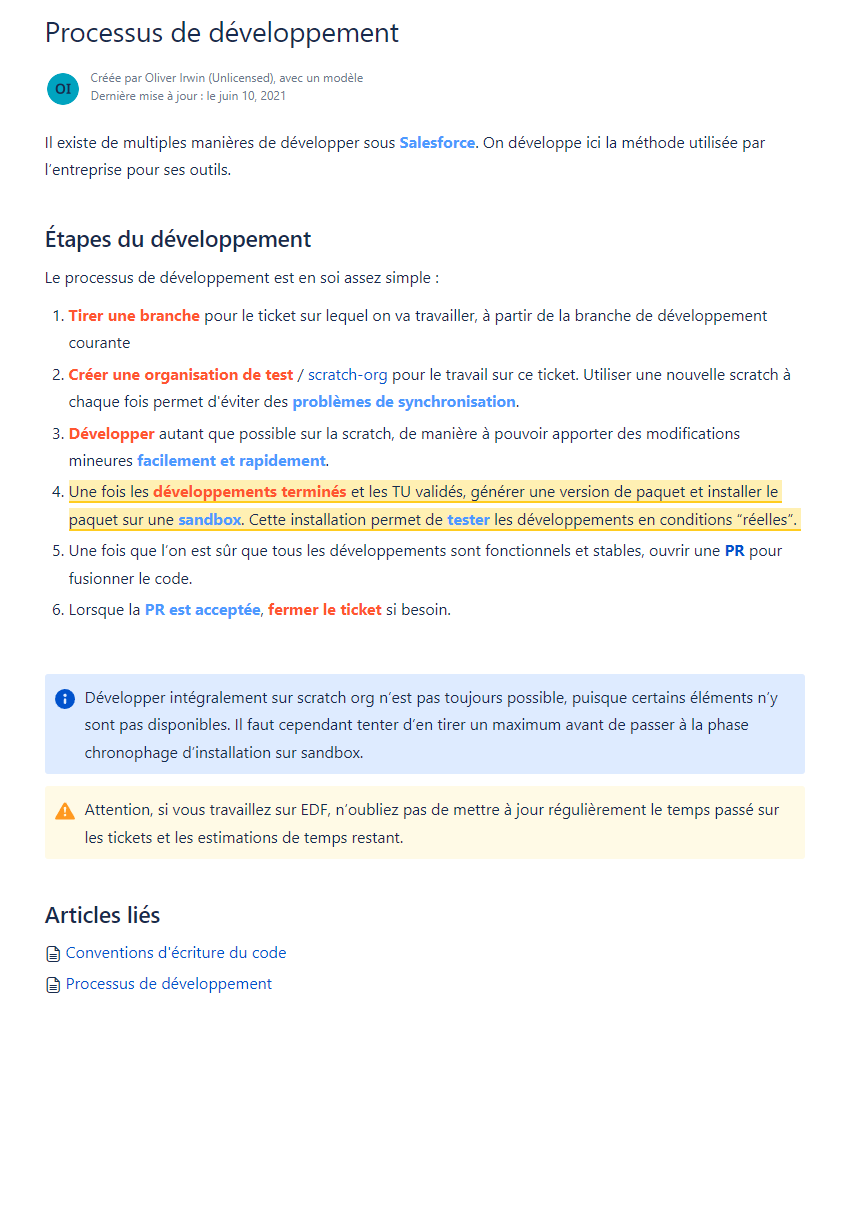
\includegraphics[width=15cm]{img/processDev.png}
  \caption{Processus de développement de\gz{}}
\end{figure}

\clearpage

\section{Utilisation de la méthode agile avec Jira}
Jira est un système de gestion de projet. \gz{} l'utilise pour gérer et planifier les tâches à réaliser dans le cadre de leurs projets. Jira possède donc un système de ticket avec lesquels l'entreprise travaille afin d'assigner les différentes tâches aux développeurs. Un ticket est composé d'un titre et d'une description devant refléter à tout moment le problème à résoudre et la solution finalement apportée. La bonne pratique pour rédiger un ticket d'anomalie est de décrire : 
\begin{enumerate}
    \item Les étapes nécessaires pour reproduire systématiquement le défaut (si défaut il y a), avec tous les éléments de contexte pertinents.
    \item Le résultat attendu
    \item Le résultat obtenu
\end{enumerate}

Chaque ticket possède un état, en effet, un ticket peut être "à faire", peut être une "idée", peut être "en cours", peut être "terminé", ou encore en "revue de code", etc. Il y a un système logique de changement d'état. On ne peut pas passer l'état d'un ticket de "à faire" à un état "terminé", il doit d'abord passer par l'état "en cours".

~\\\indent Il est possible d'estimer le temps de réalisation d'un ticket afin d'obtenir un suivi temporel des différentes tâches d'un projet, pour pouvoir par la suite mieux estimer certaines tâches. On peut également donner une priorité à une tâche. On a les différentes priorités suivantes : 
\begin{enumerate}
    \item Lowest (priorité la plus basse)
    \item Low (priorité basse)
    \item Medium (priorité moyenne)
    \item High (priorité élevée)
    \item Highest (priorité la plus élevée)
\end{enumerate}

\clearpage
 
\section{Méthodologie et étapes de développement sur Shaker Data}
 Glaz Tech +Fi suit une méthodologie de travail structurée lors du développement. Chaque tâche à accomplir est formalisée par la création d'un ticket sur Jira, détaillant la nature de la tâche. L'entreprise utilise Git, un système de contrôle de version, pour suivre et gérer les versions de leurs divers projets.

Lorsqu'un développeur est assigné à un ticket, la première étape consiste à créer une nouvelle branche à partir de la branche de développement actuelle sur Git. Cette branche est dédiée au développement en cours, permettant au développeur de travailler de manière isolée et d'éviter les conflits avec d'autres développements.

Le développeur crée ensuite une organisation Scratch pour le travail du ticket, ce qui aide à éviter les problèmes de synchronisation. Le développement se fait autant que possible sur cette Scratch Org, facilitant l'apport de modifications mineures de manière rapide et efficace.

Une fois le développement terminé et les tests unitaires du projet validés, le développeur génère une version de paquet et l'installe sur une organisation Sandbox du projet. Cette étape permet de tester les développements dans des conditions réelles et de détecter les problèmes potentiels liés au déploiement.

Avant de fusionner le code développé avec la branche de production, il est essentiel de s'assurer que tous les développements sont fonctionnels et stables. Cela implique l'exécution de l'ensemble des tests unitaires du projet pour vérifier que le travail effectué n'a pas compromis l'intégrité du projet. Si ces tests sont réussis, une Pull Request est ouverte sur Git. Une fois que la Pull Request est acceptée par le responsable du projet, le ticket peut être fermé.
 
 \begin{figure}[!ht]
  \centering
  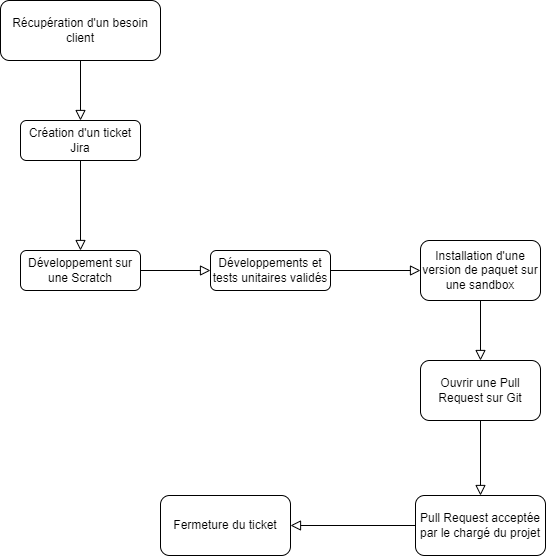
\includegraphics[width=15cm]{img/schemaEtapesDev.drawio.png}
  \caption{Schéma des étapes de développements de l'entreprise}
\end{figure}
\clearpage

\chapter{Mon travail sur le Shaker Data}
L'outil Shaker Data se compose de plusieurs pages, chacune ayant un objectif spécifique dans le processus de demande de crédit.

La page 'Dossier' : C'est la page d'accueil où l'utilisateur choisit le client qui souhaite faire un crédit.

La page 'Emprunteurs' : Sur cette page, les informations détaillées des clients qui souhaitent obtenir un crédit sont saisies. Cela comprend des informations personnelles et financières.

La page 'Situation Financière' : Comme son nom l'indique, cette page est dédiée à la saisie des actifs immobiliers du client ainsi qu'à la présentation de sa situation financière globale, y compris les détails des comptes bancaires.

La page 'Engagements Financiers' : Ici, les détails des crédits en cours du client sont saisis. Cela permet de comprendre les obligations financières existantes du client.

La page 'Projet' : Cette page est conçue pour saisir les détails des projets d'acquisition que le client souhaite réaliser. Cela peut inclure l'achat d'une maison, d'un véhicule, etc.

La page 'Récapitulatif des besoins' : Cette page fournit un résumé des besoins de financement du client, basé sur les informations saisies dans les pages précédentes.

La page 'Garanties' : Sur cette page, l'utilisateur peut choisir le type de garantie utilisé pour le crédit, qu'il s'agisse d'une \textit{hypothèque}, d'un \textit{nantissement} ou d'une \textit{caution}.

La page 'Plan de Financement' : Enfin, cette page présente les produits financiers éligibles et non éligibles pour le dossier de financement. C'est ici que la solution de financement à envoyer à la banque sera choisie.

Chaque page de l'outil Shaker Data joue un rôle crucial dans le processus de demande de crédit, permettant une collecte d'informations détaillée et une analyse approfondie pour proposer la meilleure solution de financement possible au client.

\section{Le multi-projets et la refonte graphique du plan de financement}

La page du plan de financement n'étant pas facile à comprendre au premier abord, il était nécessaire de revoir le style de la page et de mieux agencer certains éléments afin de permettre une meilleure lisibilité. Mais la problématique du multi-projets entrait également en jeu. 

Glaz Tech +Fi, à travers son outil Shaker Data, propose à ses clients de réaliser trois types de projets : 
les projets de financement immobilier, les projets de financement de \textit{SCPI} (Sociétés Civiles de Placement Immobilier) et les projets de rachat de crédits. \newline
 \indent Il arrive que les clients de Glaz Tech +Fi aient besoin de réaliser plusieurs projets simultanément. Par exemple, un client peut vouloir financer l'acquisition de parts de SCPI, mais sa situation financière actuelle peut ne pas le permettre pour que la banque accepte de financer son projet. Dans ce cas, le client a deux options : attendre une amélioration de sa situation financière ou entreprendre un projet de rachat de crédits. Si le client opte pour le rachat de crédits, il est probable qu'il souhaite ensuite obtenir un financement pour l'acquisition de SCPI une fois le rachat de crédits finalisé.

Cependant, le Shaker Data n'a pas été initialement conçu pour gérer la réalisation de plusieurs projets successifs. Il a été conçu pour financer un seul type de projet à la fois, ce qui signifie qu'il n'est pas possible de réaliser un projet de financement de SCPI et un projet de rachat de crédits simultanément. Pour pouvoir gérer ce type de dossier de financement, des améliorations doivent être apportées au Shaker Data.

Ainsi, je me suis occupé de la partie essentiellement \textit{front-end} de la page plan de financement pour cette nouvelle fonctionnalité du multi-projets.

Pour cela, une web-designeuse a pu nous aidé en réalisant la maquette par rapport à laquelle je devais me baser pour changer le style de la page. 
La voici ci-dessous.
L'introduction de la fonctionnalité permettant de gérer plusieurs projets simultanément a augmenté la complexité de l'utilisation du Shaker Data. Les utilisateurs sont passés d'un parcours où ils géraient un seul dossier à un parcours où ils doivent gérer plusieurs dossiers. Cette augmentation de la complexité a nécessité une refonte de l'interface utilisateur du Shaker Data.

En optimisant la page du plan de financement, notre objectif est d'améliorer l'expérience utilisateur et de faciliter la gestion de plusieurs projets au sein du Shaker Data.
\begin{figure}[!ht]
  \centering
  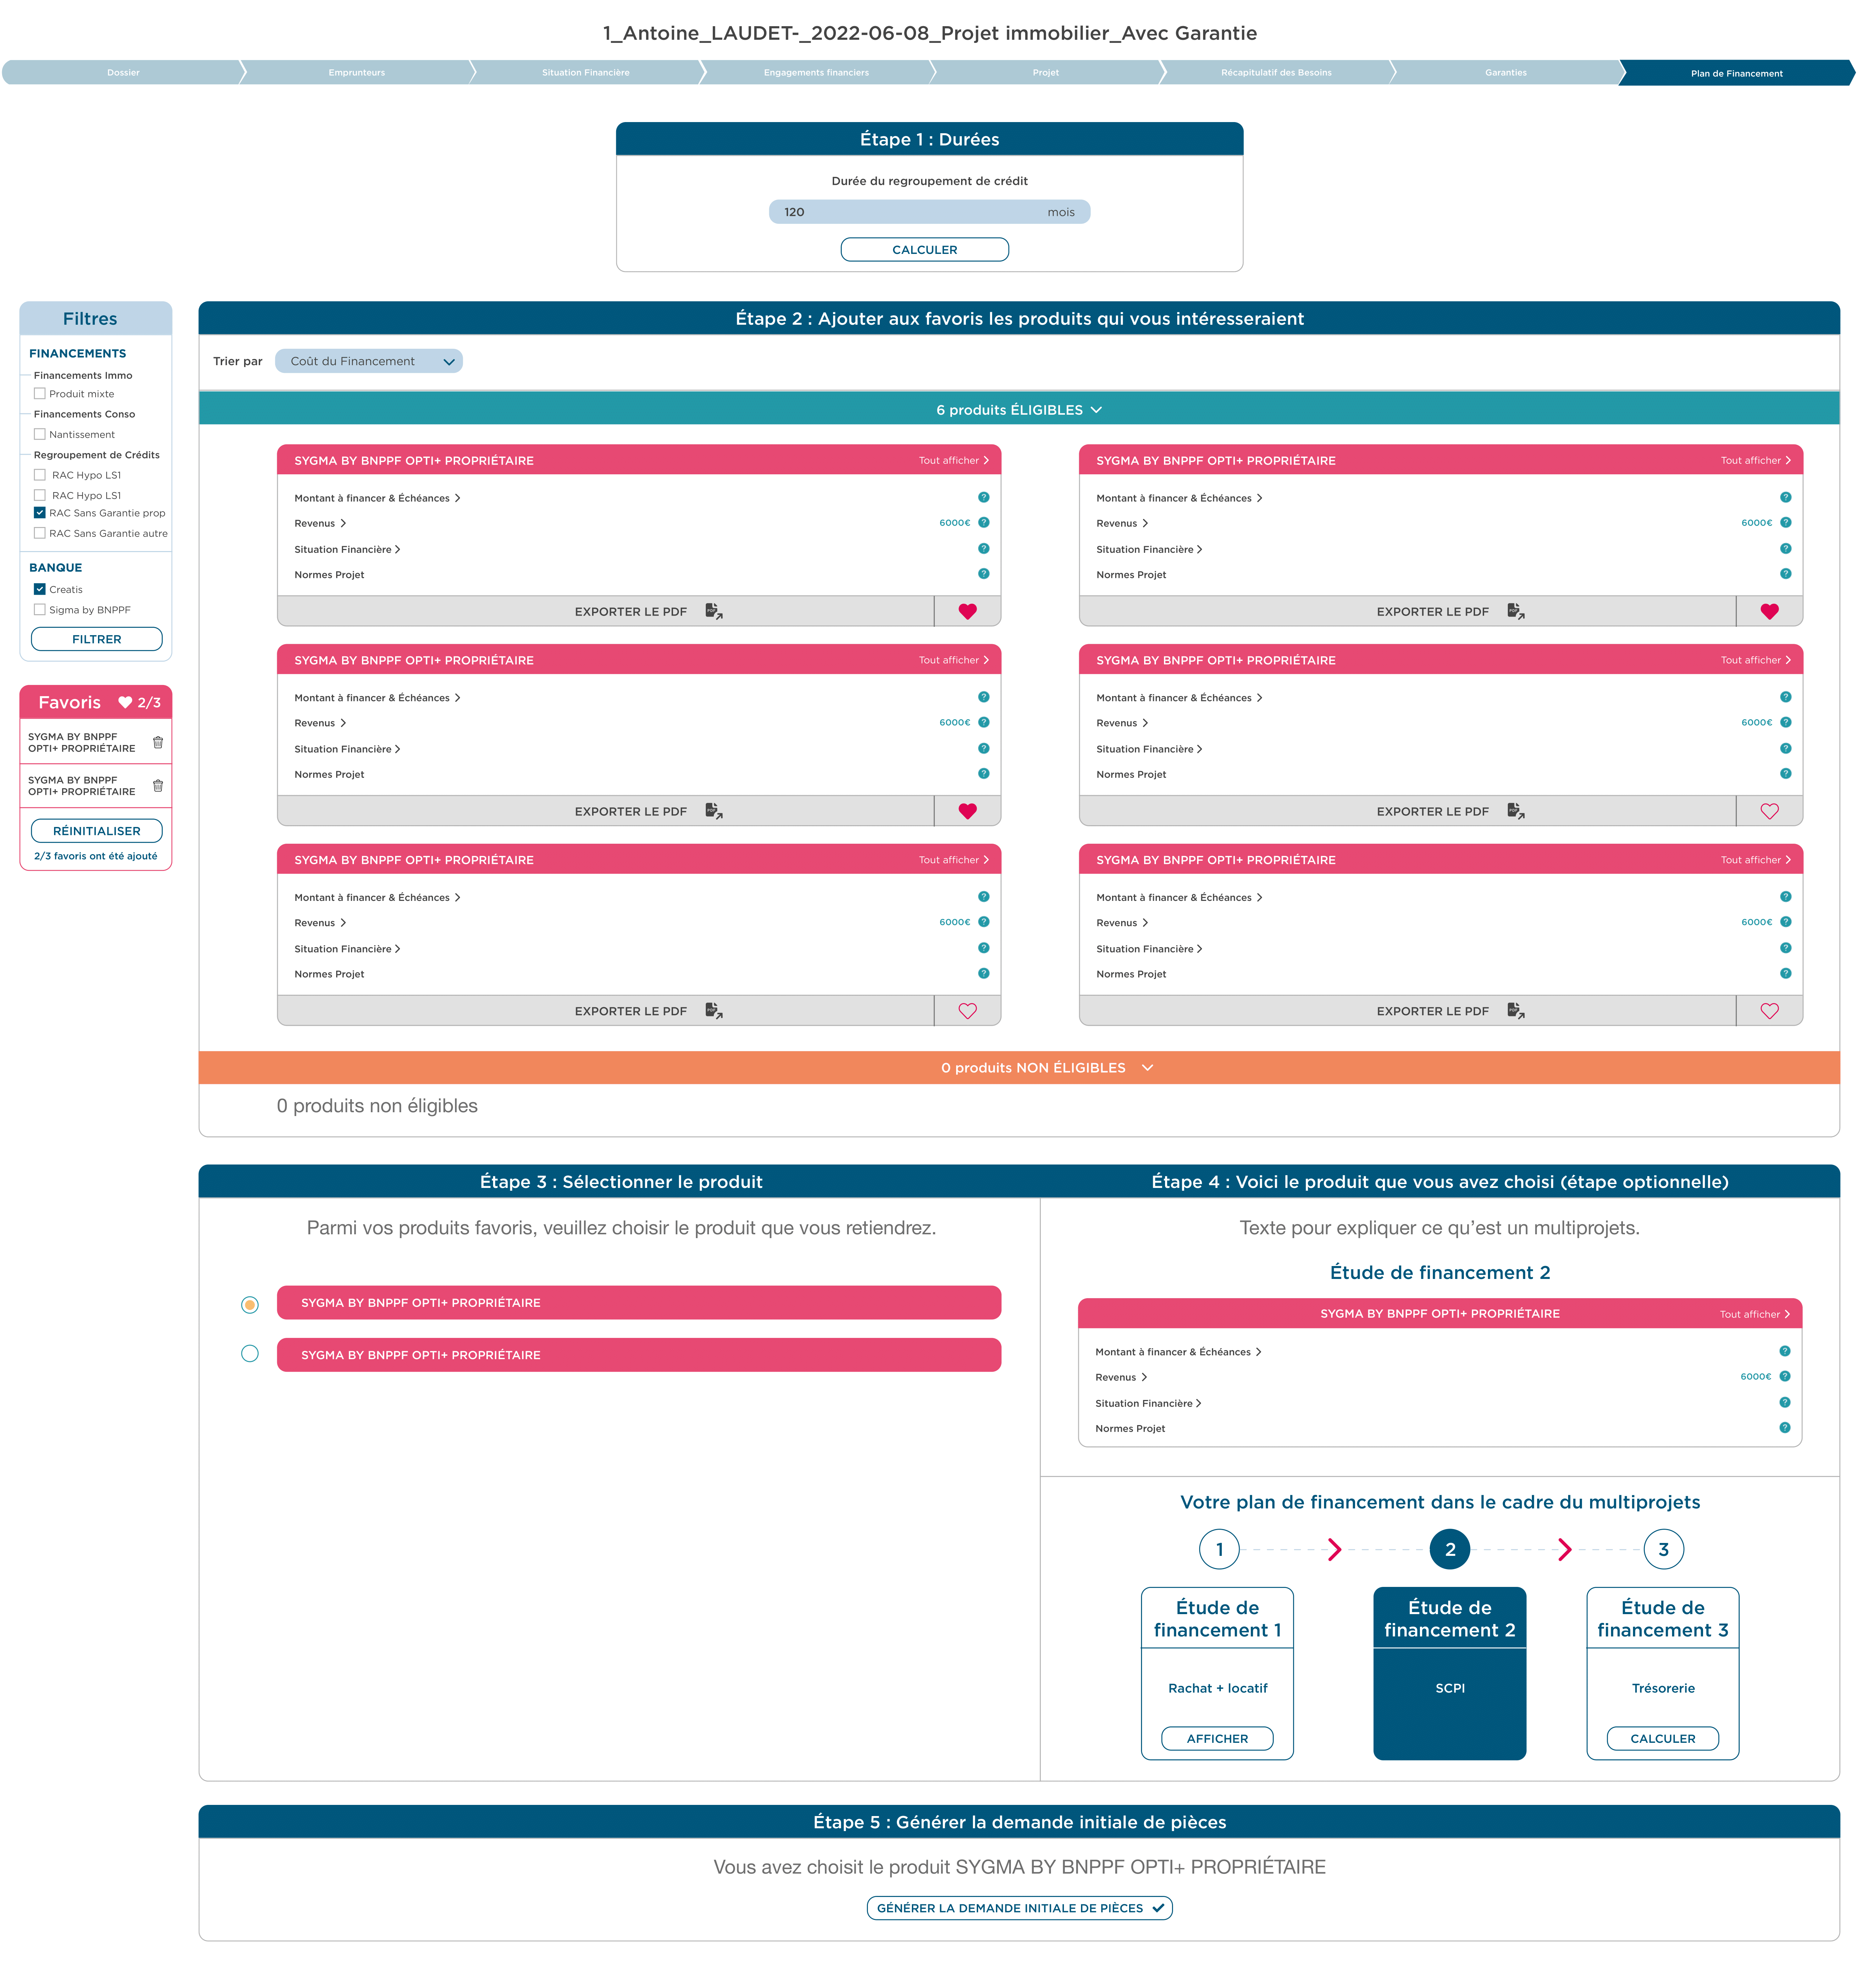
\includegraphics[width=15cm]{img/page1Maquette-1.png}
  \caption{Maquette Type de la refonte graphique}
\end{figure}

\clearpage

\subsection{La refonte des produits}
Initialement, ma tâche consistait à modifier le style des blocs de produits et leurs détails pour qu'ils se rapprochent au maximum de la maquette. Cependant, j'ai également dû intégrer la fonctionnalité des produits favoris dans cette refonte. Cette fonctionnalité permet à l'utilisateur de sélectionner jusqu'à trois produits favoris, parmi lesquels il pourra ensuite choisir celui qu'il souhaite envoyer en banque.

\begin{figure}[!ht]
  \centering
  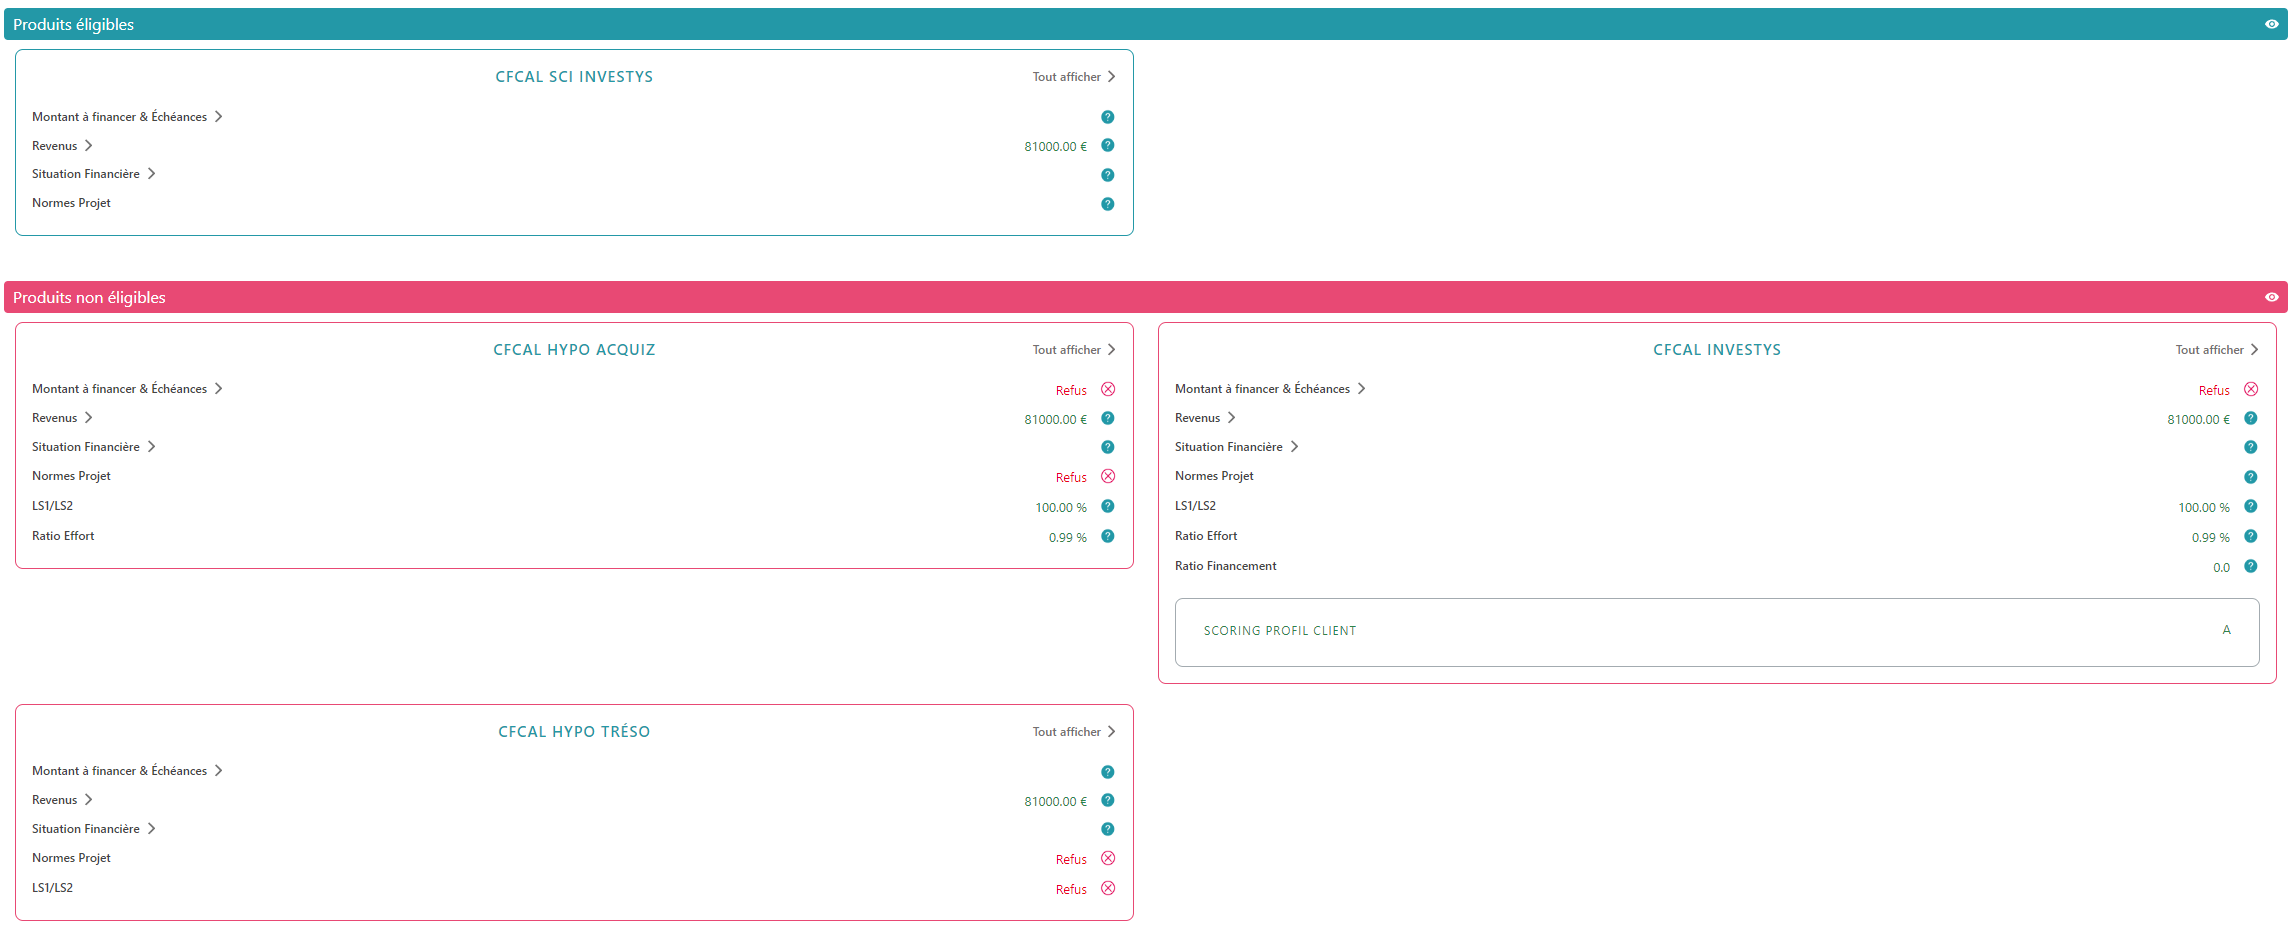
\includegraphics[width=14cm]{img/ProduitsAvant.png}
  \caption{La section des produits avant la refonte}
\end{figure}

\begin{figure}[!ht]
  \centering
  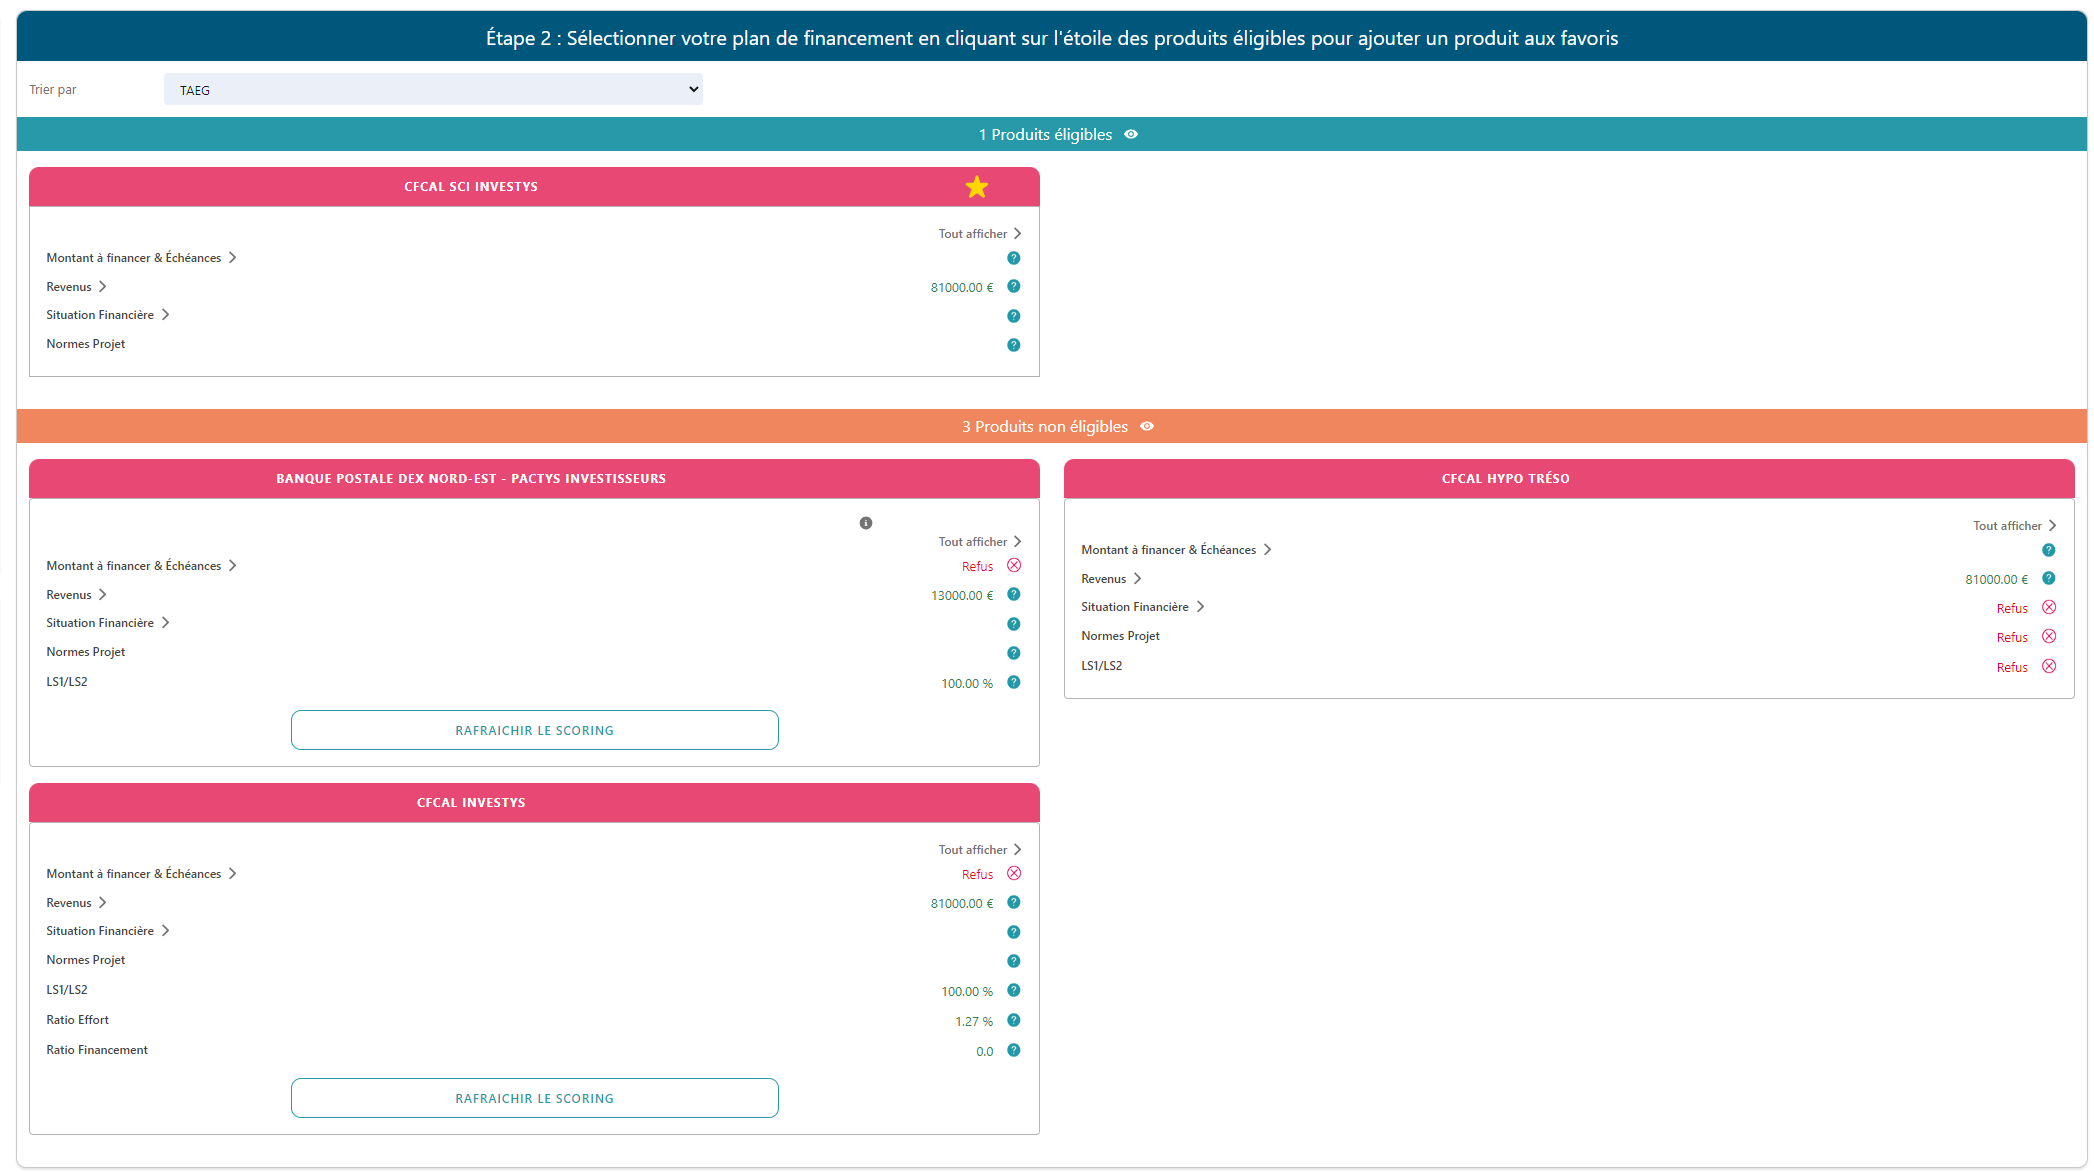
\includegraphics[width=14cm]{img/ProduitsApres.png}
  \caption{La section des produits après la refonte}
\end{figure}

La page est maintenant plus lisible et plus agréable à visualiser pour l'utilisateur.

\clearpage


.
\section{La refonte \textit{SCPI}}
Les Sociétés Civiles de Placement Immobilier (\textit{SCPI}) offrent aux investisseurs individuels une opportunité d'investir dans le secteur immobilier. En investissant dans des SCPI, les investisseurs acquièrent des parts de ces sociétés qui, à leur tour, possèdent des biens immobiliers. Les loyers générés par ces biens sont ensuite redistribués aux investisseurs proportionnellement au nombre de parts qu'ils détiennent.

L'un des principaux avantages des SCPI par rapport à l'investissement direct dans l'immobilier est qu'elles permettent aux investisseurs de bénéficier des avantages de l'immobilier sans avoir à gérer les contraintes associées à la possession d'un bien immobilier. Cela comprend la recherche de locataires, la gestion des travaux d'entretien, le traitement des impayés, et bien plus encore. Cependant, il est important de noter que les SCPI ne sont pas exemptes de risques. Leur rendement peut varier en fonction des conditions économiques générales.

Dans le Shaker Data, la gestion des SCPI a été initialement conçue pour répondre aux besoins spécifiques de notre premier mandataire, le Crédit Foncier et Communal d'Alsace et de Lorraine (CFCAL). Ce choix a été fait lors de la création de notre application pour accélérer son développement. Cependant, aujourd'hui, Glaz Tech +Fi obtient de plus en plus de mandats de banques dont les modes de fonctionnement diffèrent de celui du CFCAL. Il est donc crucial d'adapter la manière dont le Shaker Data gère le financement des SCPI. L'objectif est de rendre l'outil suffisamment flexible pour s'adapter aux différents modes de fonctionnement de nos diverses banques partenaires.

\subsection{La solution à la refonte SCPI}
Pour gérer le financement des SCPI au sein du Shaker Data, nous avons décidé d'adopter une modélisation minimale des SCPI. Cette décision a été prise en raison de la nature fluctuante et évolutive des données relatives aux différentes SCPI. Les caractéristiques des SCPI, telles que le prix d'entrée, le rendement et les conditions de souscription, peuvent varier régulièrement. Si nous avions choisi une intégration complète avec une mise à jour régulière de toutes les données des SCPI, cela aurait entraîné une complexité accrue et des contraintes de maintenance importantes.

Notre modélisation des SCPI comprend donc :
- Une table pour représenter les SCPI
- Une table pour représenter les sociétés de gestion

La table des SCPI dans notre base de données est conçue pour stocker uniquement le nom de la SCPI et être liée à une société de gestion spécifique. Son objectif principal est de fournir une référence claire aux différentes SCPI finançables par nos banques partenaires. La table des sociétés de gestion a été créée pour stocker des informations détaillées sur chaque société de gestion, y compris le nom, l'adresse, les coordonnées de contact, et d'autres informations pertinentes. Cette table nous permet de recueillir et de conserver des informations complètes sur nos fournisseurs de SCPI.

Pour faciliter la saisie des SCPI pour nos utilisateurs, nous avons restructuré l'écran pour rendre le processus de sélection de SCPI aussi intuitif que possible. Auparavant, la saisie d'un projet de SCPI était assez simple : l'utilisateur sélectionnait son projet de SCPI et indiquait le montant qu'il souhaitait investir. La banque proposait ensuite au client un type de SCPI correspondant à ses besoins. Cependant, nous avons décidé de modifier cette approche pour permettre à nos utilisateurs de choisir précisément les SCPI qu'ils souhaitent financer.

Pour ce faire, nous nous sommes inspirés de notre partenaire historique, le CFCAL. Nous avons décidé de demander à l'utilisateur de commencer par indiquer la société de gestion avec laquelle il souhaite travailler. En fournissant cette information, le Shaker Data peut proposer à l'utilisateur uniquement les SCPI proposées par la société de gestion sélectionnée. L'utilisateur peut ensuite choisir la SCPI spécifique qu'il souhaite financer.

Grâce à cette nouvelle structuration de la saisie des projets de SCPI, nous pouvons offrir à nos utilisateurs une expérience plus fluide et adaptée à leurs besoins spécifiques en matière de financement de SCPI. En leur permettant de choisir précisément la SCPI qui correspond à leurs préférences, nous améliorons leur expérience utilisateur.

\clearpage

 \begin{figure}[!ht]
  \centering
  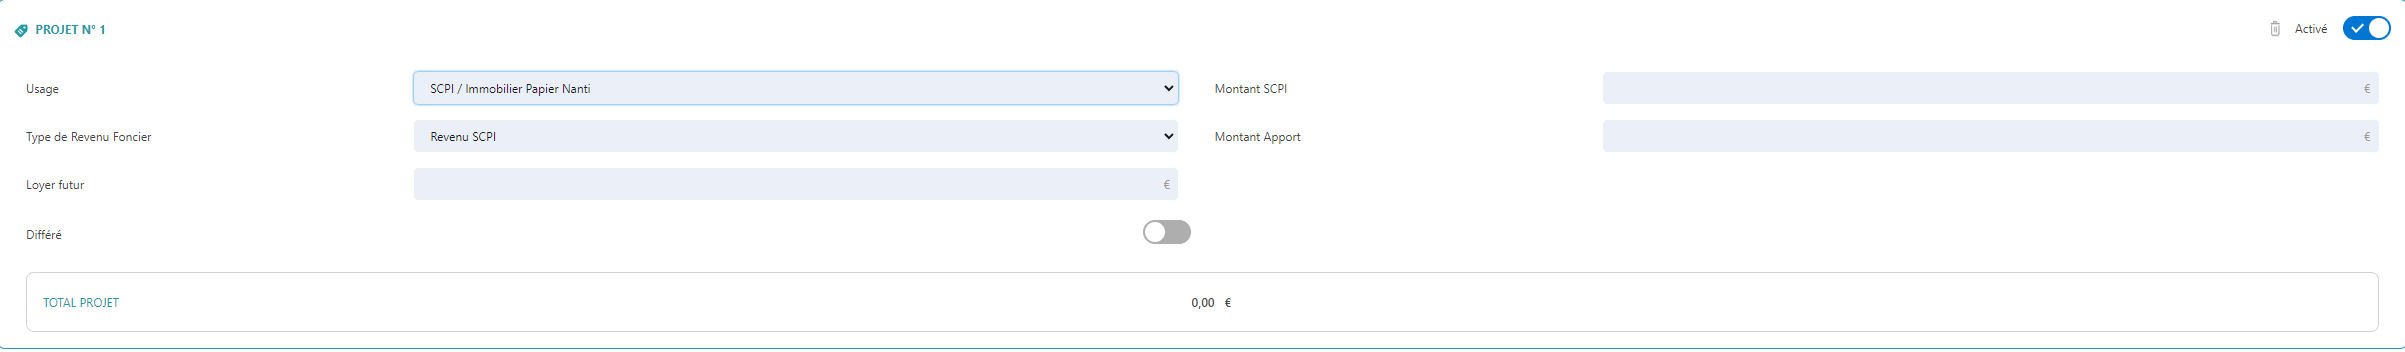
\includegraphics[width=17cm]{img/projetPageAvant.png}
  \caption{La saisie d'acquisition de SCPI avant la refonte SCPI}
\end{figure}
 \begin{figure}[!ht]
  \centering
  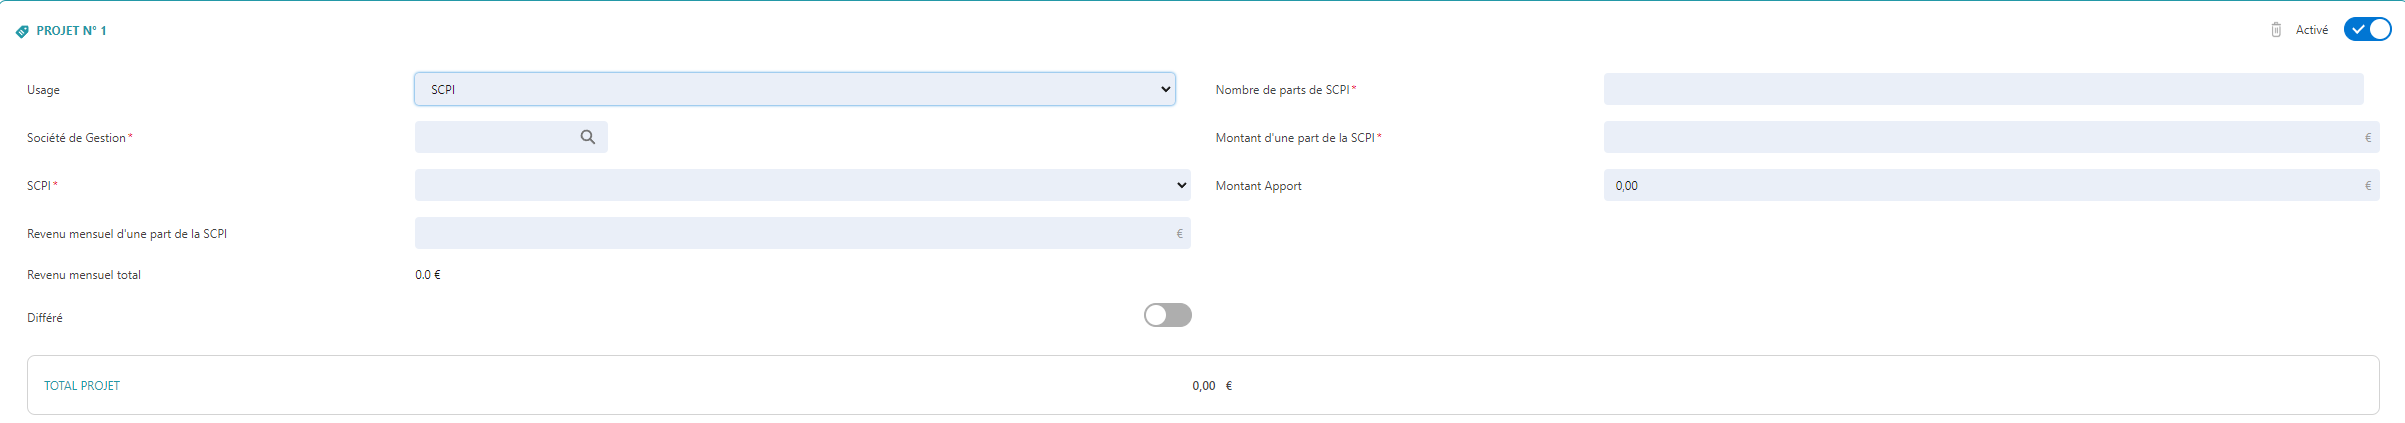
\includegraphics[width=17cm]{img/projetPageApres.png}
  \caption{La saisie d'acquisition de SCPI après la refonte SCPI}
\end{figure}
\clearpage
\clearpage



\section{Les comptes bancaires}
L'éligibilité à certains produits bancaires est souvent déterminée par la date d'ouverture du compte bancaire du client. Si le compte a été ouvert après une certaine date, le client est considéré comme un prospect, c'est-à-dire qu'il n'est pas encore un client de longue date de la banque et peut ne pas avoir accès à tous les avantages que la banque offre à ses clients plus établis.

Une des améliorations que j'ai apportées à l'outil Shaker Data est la fonctionnalité permettant de saisir les détails des comptes bancaires du client. Cette fonctionnalité facilite la collecte et l'analyse des informations bancaires du client, contribuant ainsi à une évaluation plus précise de son éligibilité aux différents produits bancaires.

Grâce à cette nouvelle saisie possible des comptes bancaires du client et de la date d'ouverture de ceux-ci, l'analyse des produits éligibles au dossier est plus fine, plus précise et se rapproche encore plus de la réalité et de l'étude de faisabilité réélle du dossier par les banques.

 \begin{figure}[!ht]
  \centering
  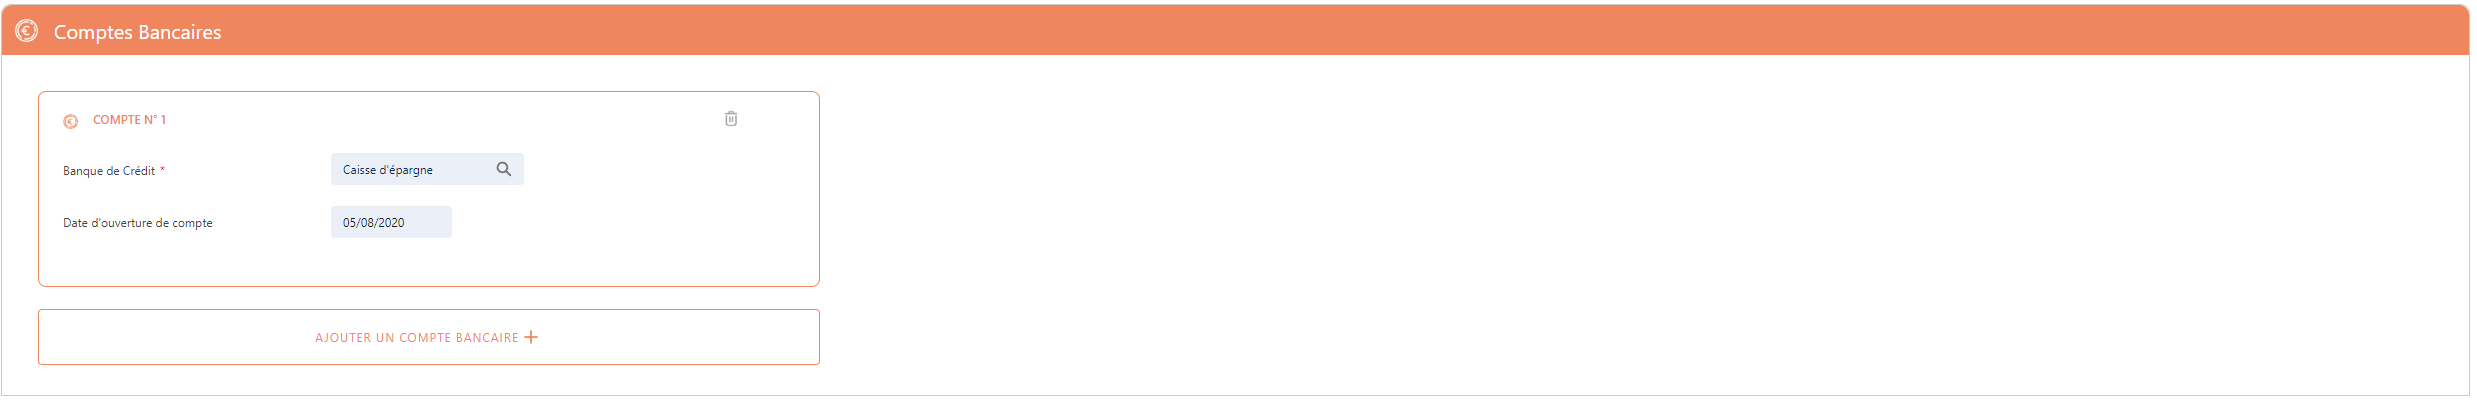
\includegraphics[width=17cm]{img/compteDeBanque.png}
  \caption{La saisie des comptes bancaires}
\end{figure}


\SpecialSection{Conclusion}
Avec l'aide des différents outils de gestion de relation et client et la plate-forme de développement de \slf{}, j'ai pu concevoir et développer, en équipe, un outil facilitant le travail des gestionnaires de patrimoine en proposant un suivi personnel et financier de leurs clients.
~\\\indent Lors de ce stage j'ai donc pu acquérir de nouvelles connaissances ainsi que de nouvelles compétences. En effet, j'ai découvert \slf{} et l'outil de gestion de relation client qu'il est, ainsi que sa plateforme de développement. En outre, j'ai pu mettre en pratique la méthode agile ainsi que les bonnes pratiques de code. En effet, ayant travaillé au long du stage au sein d'une équipe de développeurs, j'ai été forcément amené à retravailler du code qui n'était pas le mien. C'est grâce à cela que j'ai compris combien il était important de structurer et de documenter son code, comme j'ai pu l'apprendre lors du DUT, afin que les prochaines personnes qui le retravaille puisse le comprendre facilement. Cela permet un gain de temps non négligeable sur les développements de chacun. Grâce à l'apprentissage de l'outil Git lors de mes études, j'ai pu facilement assimiler son utilisation au sein de l'entreprise. Mais aussi, l'enseignement de la méthode agile m'a permis de rapidement comprendre la méthodologie de travail de \gz{} à travers sa planification et sa quantification du temps de travail des tâches de chacun. Pour finir sur ce parallèle entre mon stage et ma formation à l'IUT, j'ai pu réutiliser mon apprentissage de différents langages lors du DUT. J'ai pu utilisé du JavaScript, de l'HTML et du CSS mais il y a également l'enseignement du Java que j'ai pu retranscrire en programmant en Apex.
~\\\indent Cette expérience m'a conforté dans l'idée de vouloir continuer l'an prochain vers une licence professionnelle dans le développement Web en alternance, afin de pouvoir continuer mes études tout en acquérant de l'expérience professionnelle. 

\bibliographystyle{myunsrt}
\small
\bibliography{rapport}
Site d'une agence d'intérim/cabinet de recrutement https://www.manpower.fr/ \newline
https://www.journaldunet.fr/ \newline
wikipedia.org \newline
https://developer.mozilla.org/


\Annex{Annexe 1}
\newpage
\Annex{Glossaire}
    \textbf{Gestionnaire de patrimoine} : Le conseiller de gestion en patrimoine gère les actifs de ses clients. C’est un spécialiste de l’investissement qui a pour rôle de fournir des programmes sur mesure à ses clients pour préserver ou accroître leur patrimoine.\newline
    
   ~\\\indent \textbf{Courtier immobilier} : Un courtier en financement immobilier est un intermédiaire entre une banque et un particulier en quête d’un crédit immobilier pour financer l’acquisition de son bien.\newline


    ~\\\indent \textbf{FinTech} est un terme créé par la fusion des mots "finance" et "technologie". Il désigne une entreprise de type start-up, proposant des services financiers en s'appuyant sur les nouvelles technologies numériques. \newline


    ~\\\indent Un \textbf{apporteur d'affaires} est une personne qui met en relation des personnes qui souhaitent réaliser entre elles des opérations commerciales. Pour l'entreprise en l'occurrence, c'est lui qui va apporter les différents dossiers de ses clients, afin que nous les traitons.\newline


    ~\\\indent \textbf{Composant standard} est un élément développé par \slf{} que l'on peut réutiliser afin de concevoir des pages web sur celui-ci.\newline


     ~\\\indent Les outils \textbf{Low Code/No Code} permettent de créer des applications (mobile ou web) ou d’automatiser des processus sans nécessairement maîtriser toutes les étapes de programmation bien souvent complexes. Ces outils sont basés sur les trois principes suivants: 
    \begin{enumerate}
        \item conception d’applications directement via des modèles
        \item La possibilité de glisser-déposer des composants applicatifs pour former des pages web
        \item génération automatique de lignes de code
        \item programmation visuelle
    \end{enumerate}
    
    ~\\\indent \textbf{Financial Services Cloud} (FSC) est une solution de gestion de la relation client (CRM) qui aide les
entreprises du secteur financier à gérer les références, les documents, les tâches et plus
encore. En résumé c'est une licence payante additionnelle de \slf{} qui rajoute des
fonctionnalités afin d'améliorer la gestion de relation client.\newline


    ~\\\indent Les \textbf{organisations Sandbox} sont des environnements \slf{} se rapprochant le plus de l'environnement de production, en effet, la Sandbox copie l'organisation de production en omettant les données présentes sur celle-ci. Cela permet donc de tester les développements en conditions réelles avant de réellement les déployer en production. Une organisation Sandbox peut être effacée lorsqu'on le souhaite.\newline
    
    ~\\\indent Les \textbf{organisation scratch}sont des organisations vides contenant aucune donnée et qui sont automatiquement effacées dans un délai de 30 jours maximum. Ce sont des environnements jetables dédié au développement, chaque développeur travaille seul sur sa scratch.\newline


    ~\\\indent Une \textbf{opportunité} est un objet sur \slf{} qui représente un dossier, qui définit une opportunité d'investissement pour le client, on peut y retrouver son sujet, sa probabilité de réussite (selon le gestionnaire de patrimoine), ou encore le montant de l'investissement prévu.\newline


   ~\\\indent \textbf{FormAssembly} est la solution de formulaire nº1 pour \slf{} conçue pour aider les équipes à rationaliser les processus complexes et à générer des conversions de formulaires de qualité.\newline


   ~\\\indent Les \textbf{LWC} (Lightning Web Components) sont des éléments HTML personnalisés qui utilise de l'HTML, du CSS et du JavaScript.\newline

  ~\\\indent  Les \textbf{meta-données} sur \slf{} sont des fichiers \textit{XML} qui représente les différents éléments qui le compose, tels que les objets, les présentations de page, les LWC, etc. Les meta-données sont donc des données qui décrivent des données.\newline


    ~\\\indent \textbf{Git} est un système de contrôle de version. Il s’agit d’un outil de développement qui aide une équipe de développeurs à gérer les changements apportés au code source au fil du temps, et à garder une trace de ceux-ci.\newline


 ~\\\indent \textbf{Branche (Git)} : Presque tous les système de contrôle de version tels que Git proposent une certaine forme de gestion de \textbf{branches}. Créer une branche signifie diverger de la ligne principale de développement et continuer à travailler sans impacter cette ligne.\newline


 ~\\\indent Les \textbf{pull requests} sur git sont une fonctionnalité facilitant la collaboration des développeurs. Elles fournissent une interface Web qui permet discuter des changements proposés avant de les intégrer au projet officiel. Une fois qu'il effectué une revue de code de la pull request, le chargé de projet s'occupe de l'accepter, ou décide demander des modifications sur celle-ci.
\newline

 ~\\\indent Le \textbf{refactoring de code} consiste à améliorer le code source d’une application informatique en le modifiant sans ajouter de nouvelles fonctionnalités et sans fixer de bugs. Cette amélioration peut consister à de la simplification pour faciliter sa maintenance ou le rendre plus générique. Le tout sans modifier le comportement fonctionnel de la solution informatique.\newline

 ~\\\indent \textbf{XML} est un langage de balisage créé pour définir une syntaxe de codage de documents que les humains et les machines peuvent lire. Pour ce faire, il utilise des balises qui définissent la structure du document, ainsi que la manière dont le document doit être stocké et transporté.\newline


     ~\\\indent Les feuilles de style en cascade, généralement appelées \textbf{CSS} de l'anglais Cascading Style Sheets, forment un langage informatique qui décrit la présentation des documents HTML et XML. Il permet ainsi de décorer ces dernières.\newline


     ~\\\indent \textbf{HTML}
    description=Le HyperText Markup Language, généralement abrégé HTML ou, dans sa dernière version, HTML5, est un langage informatique conçu pour représenter les pages web.\newline



     ~\\\indent \textbf{Javascript} est un langage de programmation qui permet d'implémenter des mécanismes complexes sur une page web. À chaque fois qu'une page web fait plus que simplement afficher du contenu statique — afficher du contenu mis à jour à des temps déterminés, des cartes interactives, des animations 2D/3D, des menus vidéo défilants, ou autre, JavaScript a de bonnes chances d'être impliqué.


\end{document}

